\documentclass[11pt,a4paper]{article}
\usepackage[T1]{fontenc}
\usepackage{lmodern}
\usepackage{microtype}
\usepackage[margin=2.2cm]{geometry}
\usepackage{amsmath}
\usepackage{graphicx}
\usepackage{booktabs}
\usepackage{tabularx}
\usepackage{array}
\usepackage[table]{xcolor}
\usepackage{enumitem}
\usepackage{placeins}
\usepackage[font=small,labelfont=bf]{caption}
\usepackage[most]{tcolorbox}
\usepackage[colorlinks=true,linkcolor=blue!50!black,urlcolor=blue!50!black]{hyperref}

\graphicspath{{figures/}}
\setlist{nosep,leftmargin=*}
\setlength{\parskip}{4pt}
\setlength{\parindent}{0pt}
\newcolumntype{L}{>{\raggedright\arraybackslash}X}
\newtcolorbox{keybox}[1]{colback=blue!3,colframe=blue!40!black,boxrule=0.5pt,arc=1pt,
  left=6pt,right=6pt,top=4pt,bottom=4pt,title=#1,fonttitle=\bfseries\small}
\newcommand{\code}[1]{\texttt{\footnotesize #1}}

\title{\textbf{Hybrid-OED: status after the October 2026 extension}\\[4pt]
\large From a 2-D acoustic proof of concept towards online OED with the LDV in the loop}
\author{Working notes, 25 October 2026 (updated 26 October: OED on the LDV setup)}
\date{}

\begin{document}
\maketitle

\begin{keybox}{Bottom line}
\begin{itemize}
  \item \textbf{Compute is no longer a constraint.} With rematerialisation (\code{jax.checkpoint}) the nested
        FWI--OED hypergradients fit on one GPU; the full workshop-paper experiment runs in about 22 minutes
        instead of 4.2 hours and reproduces Table~1.
  \item \textbf{Validated fast plate models exist for both wave families.} Plane stress for in-plane S0/SH0
        (misfit 0.2--0.3 against Salvus 3-D) and Mindlin for out-of-plane A0 (about 0.15 against 3-D), solving in
        1--10~s on the GPU.
  \item \textbf{The real LDV scan is explained.} It is A0-dominated (only the out-of-plane channel is usable).
        Salvus 3-D with a bonded 10~mm steel cube and PMMA attenuation (Q~$\approx$~40) fits it to 0.33; a
        Mindlin plate with damping and a rigid-body cube fits it equally well (0.31/0.33) at a tenth of the cost.
  \item \textbf{OED with re-acquisition works end to end} (illumination design, Salvus as the ``lab''), with
        modest gains so far (single run).
  \item \textbf{OED on the LDV setup runs on real data} (Section~\ref{sec:oed-ldv}): blind Mindlin FWI of a mass map
        finds the cube from the full scan, and the online loop with 30 LDV points runs against a Mindlin lab, a Salvus
        3-D lab and a \emph{replay lab} that returns real LDV traces. Illumination design raises the recovered mass
        at the cube in all three labs, but on real data spurious anomalies at the scan edge dominate, and a single
        transducer leaves a streak along the source--cube line.
  \item \textbf{Next:} revise the experiment before going further (Section~\ref{sec:next-experiment}): a more
        realistic defect, several transducer positions, full metadata and a defect-free reference scan. Then run the
        multi-seed virtual-lab study and the live loop. The paper should claim scan-time reduction for defect
        characterisation.
\end{itemize}
\end{keybox}

\setcounter{tocdepth}{1}
\tableofcontents
\clearpage

%======================================================================
\section{What was done, at a glance}
\begin{table}[h]
\centering\small
\begin{tabularx}{\textwidth}{@{}>{\raggedright\arraybackslash}p{2.9cm}L>{\raggedright\arraybackslash}p{3.9cm}@{}}
\toprule
Topic & Result & Code / results \\
\midrule
PINN / FBPINN instead of FWI & Ruled out: the network can represent the wavefield (2.5\,\% error when fitted to data) but physics-loss training does not find it (62\,\%); minutes per solve vs 0.03~s for FD. & \code{src/pinn\_feasibility/} \\
Remat + GPU & Memory 64~GiB $\to$ 3--6~GiB, identical gradients ($\sim$$10^{-6}$); paper experiment 4.2~h $\to$ 22~min; Table~1 reproduced (max.\ per-run MSE difference 0.3\,\%). & \code{src/remat/} \\
Old Salvus data & Produced by a different run than the stored mesh (hash mismatch); contains SH0 and S0; the notebook's acoustic comparison was $\sim$30~$\mu$s misaligned. & \code{src/elastic/README.md} \\
Salvus 3-D benchmark & Free 0.6~m PMMA plate, known inclusion and sources; 24 runs in 2~min on the GPU. & \code{src/salvus\_plate/} \\
Plane stress (S0/SH0) & Free-edge solver; 0.18 (early) / 0.27 (1~ms) against Salvus with an S0 dispersion correction. & \code{src/elastic/} \\
JAX 3-D elastic & Free-plate FD solver; 0.03 / 0.10 against Salvus; 50~s per solve. & \code{src/elastic/elastic3d.py} \\
FWI with model error & Dense receivers + TV: 6.8~m/s vs 5.3 (inverse crime); 31 diagonal receivers: 12.0 vs 12.3 (geometry-limited). & \code{src/elastic/invert\_plate.py} \\
OED loop, Salvus as lab & Illumination design $\to$ new Salvus run $\to$ FWI; $-$11 to $-$12\,\% model error mid-run, $-$5\,\% at the end (one run). & \code{src/oed\_plate/} \\
LDV data & No metadata; out-of-plane SNR $\approx$ 90, in-plane channels are cross-talk; A0 of 10~mm PMMA. & \code{src/ldv\_assessment/} \\
Mindlin (A0) & Shear factor matched to exact A0 dispersion (textbook value 1--2\,\% too slow); 0.16--0.20 against 3-D. & \code{src/elastic/mindlin.py} \\
LDV explained & Salvus: steel cube + Q = 40 $\to$ 0.33. Mindlin + damping + rigid cube (6~mm effective footprint) $\to$ 0.31/0.33. & \code{src/ldv\_assessment/} \\
Static FWI on the LDV scan & Rigid-cube search: best at ($-18$, $-4$)~mm, 2~mm from the Salvus fit. Blind mass map: held-out misfit 0.48 $\to$ 0.28; cube found, plus an edge artefact. & \code{src/ldv\_inversion/} \\
OED loop on the LDV setup & 30 LDV points, Mindlin FWI; Mindlin, Salvus and replay (real data) labs. Illumination raises the mass at the cube in all labs; real data show edge artefacts. & \code{src/oed\_ldv/} \\
\bottomrule
\end{tabularx}
\end{table}

All new code lives in new folders; the scripts and conda environment used for the workshop paper are unchanged.
Misfits in this report are relative L2 errors of waveforms unless stated otherwise.

%======================================================================
\section{Compute: rematerialisation and GPU}
Differentiating the design objective through $K=20$ unrolled FWI updates stores every wavefield state of every forward
and adjoint simulation. Wrapping each FWI update in \code{jax.checkpoint} stores only its input (the model) and
recomputes the update during the backward pass. The illumination objective was treated the same way (sources one at
a time, probes in batches).

\begin{figure}[h]
\centering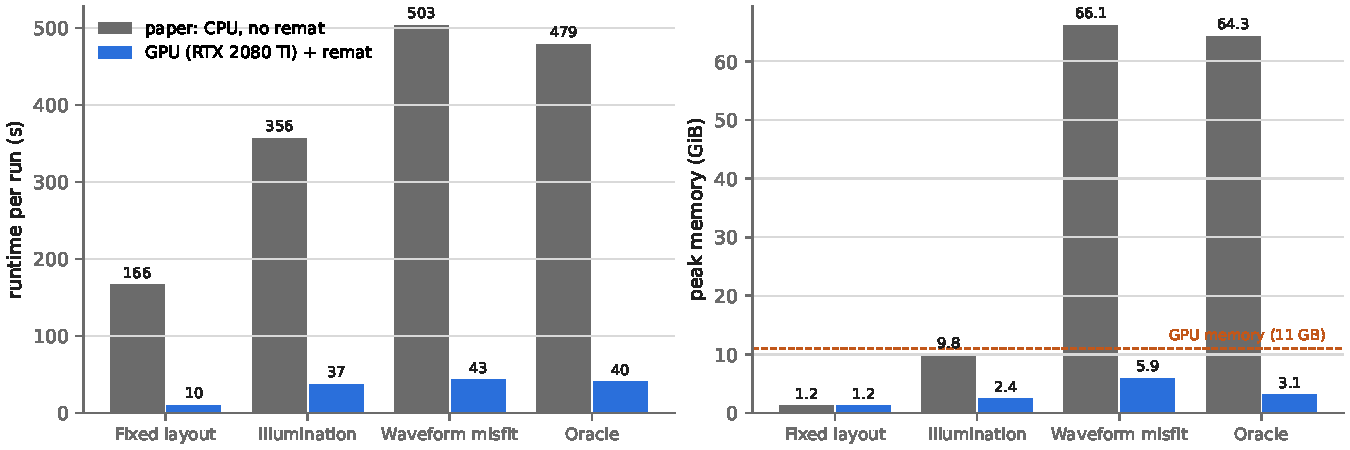
\includegraphics[width=\textwidth]{remat.pdf}
\caption{Full multi-seed experiment of the workshop paper (10 repetitions, same seeds). Left: runtime per run;
right: peak memory. The paper versions of the FWI-differentiated objectives need 64--66~GiB and do not fit the
11~GB GPU; with remat they need 3--6~GiB.}
\end{figure}

\begin{table}[h]
\centering\small
\resizebox{\textwidth}{!}{\begin{tabular}{@{}lcccc@{}}
\toprule
Method & MSE paper (CPU) & MSE GPU + remat & Improvement paper / GPU & Max.\ per-run MSE difference \\
\midrule
Fixed layout & $3358.9 \pm 65.5$ & $3358.9 \pm 65.5$ & -- & 0.000\,\% \\
Illumination & $2796.2 \pm 274.6$ & $2796.2 \pm 274.7$ & 16.7 / 16.7\,\% & 0.005\,\% \\
Waveform misfit & $3041.6 \pm 125.4$ & $3041.3 \pm 125.9$ & 9.4 / 9.4\,\% & 0.30\,\% \\
Oracle & $2732.3 \pm 242.4$ & $2732.3 \pm 242.4$ & 18.6 / 18.6\,\% & 0.004\,\% \\
\bottomrule
\end{tabular}}
\caption{The GPU + remat runs reproduce the published results. Consequence for the paper: the memory column of
Table~1 is no longer an intrinsic property of the methods.}
\end{table}

\textbf{PINNs.} Replacing FWI by (FB)PINNs was tested on the scattered-field problem: physics-loss training plateaued
at 62\,\% error after 17 minutes (with causal time-marching), while the same FBPINN fitted to the reference field reached
2.5\,\%. Together with the 0.03~s cost of an FD solve on GPU, this ruled the approach out.

\FloatBarrier
%======================================================================
\section{Plate physics: three solver families against Salvus 3-D}
To move from the 2-D acoustic proxy to plates, a fully specified Salvus benchmark was built: a free (non-absorbing)
0.6~m~$\times$~0.6~m~$\times$~10~mm PMMA plate (vp 2730, vs 1340~m/s, $\rho$ 1180~kg/m$^3$), a 60~mm soft inclusion,
12 in-plane point forces at mid-plane, a 25~kHz Ricker, and 3481 top-surface receivers. A second set of events uses
out-of-plane forces (A0). All runs use the GPU (new SalvusFlow site \code{local\_gpu}).

\begin{figure}[h]
\centering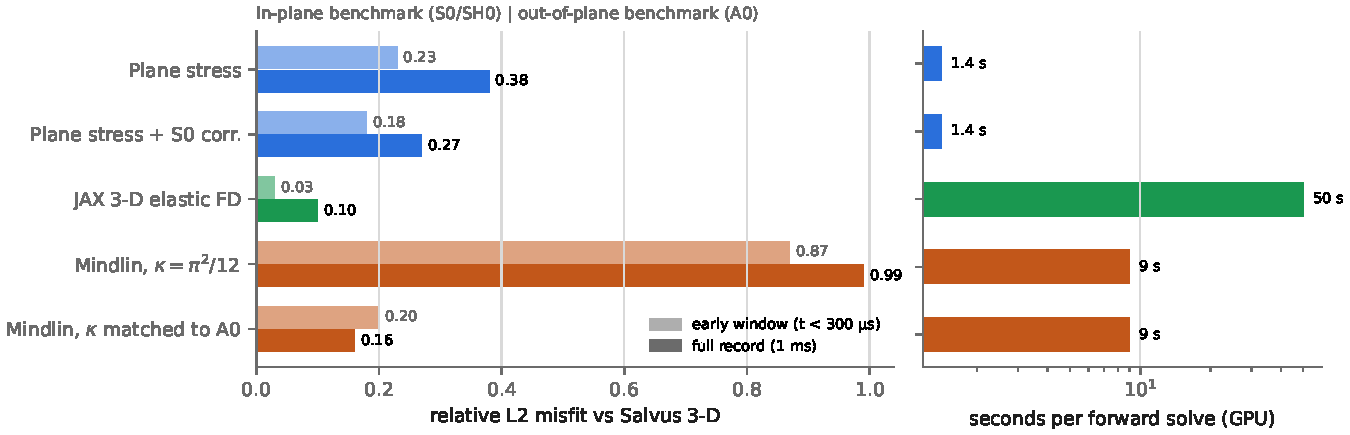
\includegraphics[width=\textwidth]{forward_models.pdf}
\caption{Accuracy and cost of the JAX solvers against Salvus 3-D. Plane stress and the 3-D FD solver are scored on
the in-plane benchmark, Mindlin on the out-of-plane (A0, mid-plane force) benchmark. The two corrections that matter:
the S0 dispersion correction for plane stress and the A0-matched shear factor $\kappa$ for Mindlin.}
\end{figure}

\begin{figure}[h]
\centering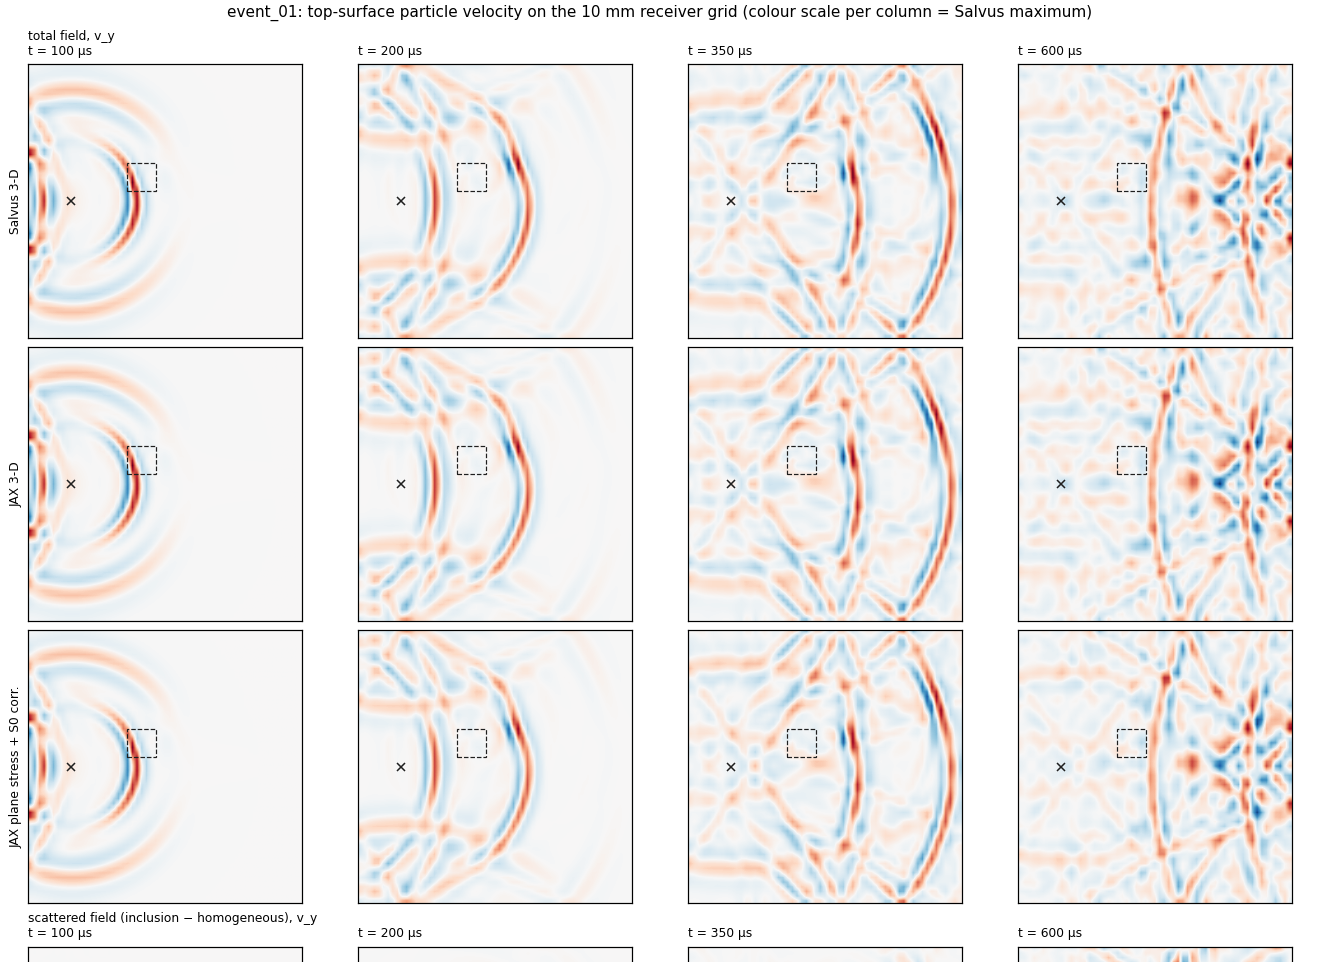
\includegraphics[width=\textwidth]{wavefield_snapshots.png}
\caption{Top-surface $v_y$ for one in-plane event (rows: Salvus 3-D, JAX 3-D, JAX plane stress with S0 correction).
Direct waves, edge reflections and the field scattered by the inclusion agree closely.}
\end{figure}

\begin{figure}[h]
\centering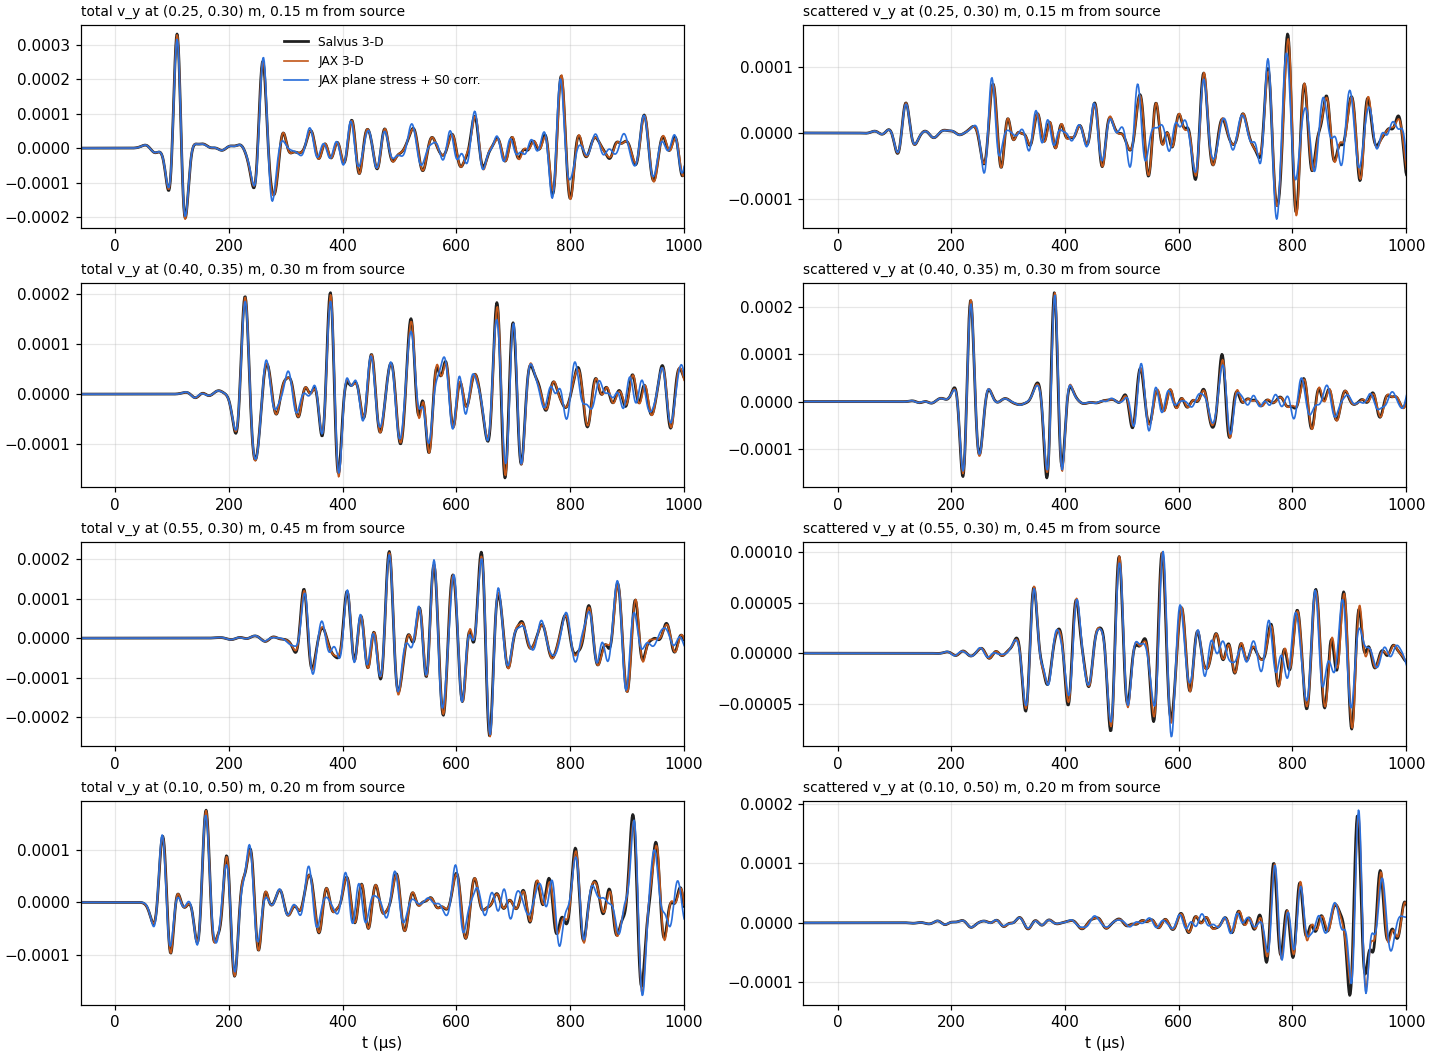
\includegraphics[width=\textwidth]{wavefield_traces.png}
\caption{Total and scattered traces at four receivers (black: Salvus 3-D, orange: JAX 3-D, blue: plane stress + S0
correction). JAX 3-D lies on Salvus; plane stress drifts slightly in phase in the late reverberations.}
\end{figure}

\begin{table}[h]
\centering\small
\resizebox{\textwidth}{!}{\begin{tabular}{@{}lccc@{}}
\toprule
Model & What it represents & Error vs 3-D & Cost / solve \\
\midrule
Plane stress (+ S0 correction) & S0, SH0 (in-plane) & 0.18--0.27 & 1.4~s \\
Mindlin ($\kappa$ matched, damping, rigid masses) & A0 (out-of-plane) & 0.14--0.20 & 9~s \\
JAX 3-D FD & everything & 0.03--0.10 & 50~s \\
Salvus 3-D (spectral elements) & everything, attenuation, 3-D attachments & reference & 6--80~s \\
\bottomrule
\end{tabular}}
\caption{Model hierarchy. The 3-D solvers are too slow for nested OED (hours per run); the plate models are fast
enough and have known errors.}
\end{table}

\FloatBarrier
%======================================================================
\section{Inversion with model error (Salvus data, plane-stress solver)}
FWI of the Salvus in-plane data with the plane-stress solver (vs on a 5~mm grid, Adam, 4 sources).

\begin{figure}[h]
\centering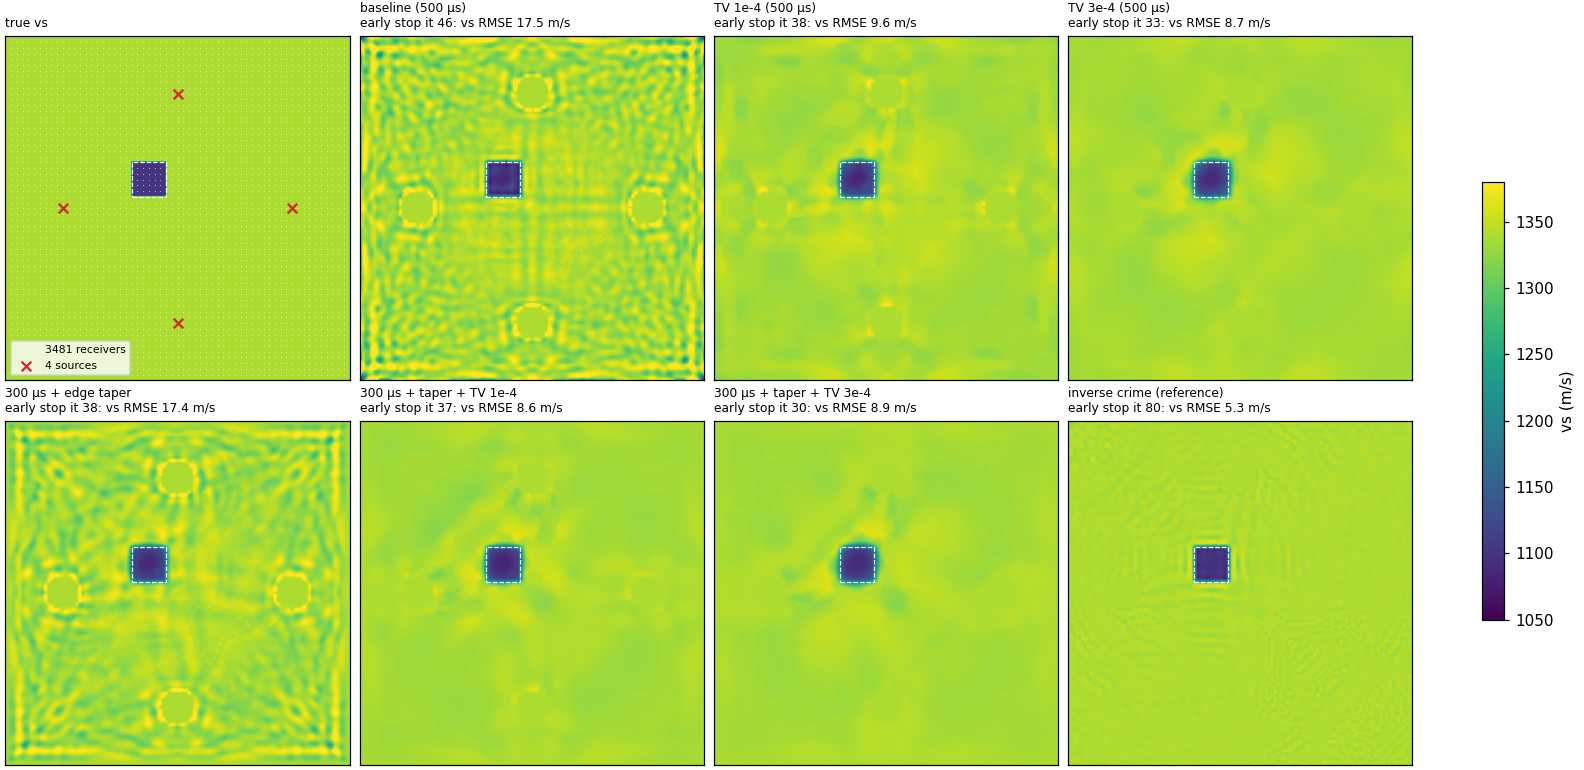
\includegraphics[width=\textwidth]{regularisation_maps.png}
\caption{Dense receivers (3481, white dots). Without regularisation the model error turns into background artefacts
(vs RMSE 20.5~m/s); total-variation regularisation removes most of them (6.7--7.7~m/s), close to the inverse crime
(5.3~m/s).}
\end{figure}

\begin{figure}[h]
\centering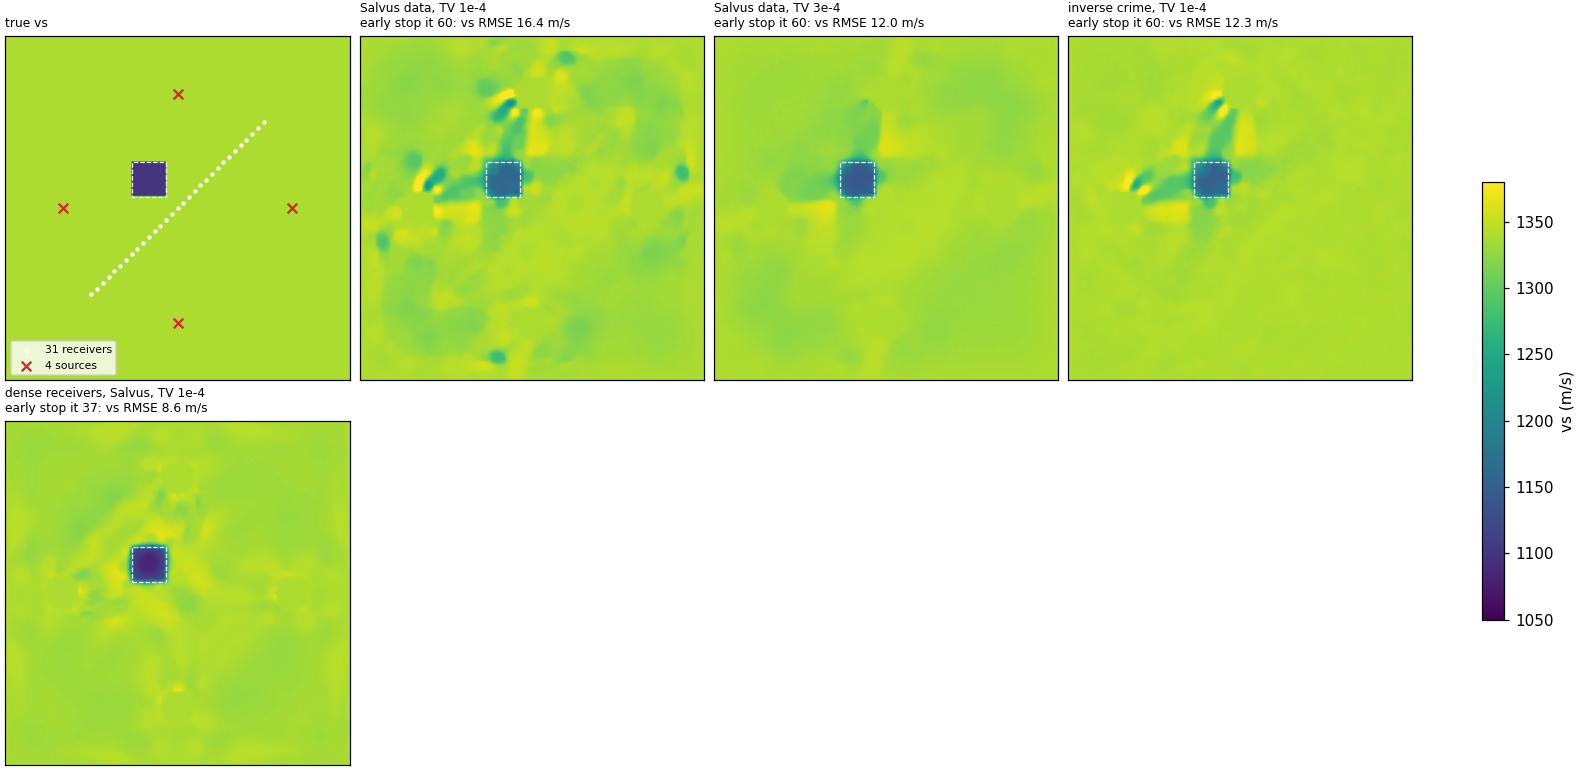
\includegraphics[width=\textwidth]{diagonal_maps.png}
\caption{31 receivers on the paper's diagonal. The inclusion is detected but smeared (about 70\,\% of its contrast);
with Salvus data and TV $3\times10^{-4}$ the error (12.0~m/s) equals the inverse crime (12.3~m/s): with sparse
receivers, the geometry, not the model error, limits the result.}
\end{figure}

\begin{table}[h]
\centering\small
\resizebox{\textwidth}{!}{\begin{tabular}{@{}lccc@{}}
\toprule
Inversion & vs RMSE (start 23.7 m/s) & Inclusion vs (true 1108) & Background std \\
\midrule
Dense, no regularisation, 80 it. & 20.5 (17.5 with early stop) & 1124 & 17.2 \\
Dense, TV, 300~$\mu$s window, edge taper & 6.8 & 1121 & 7.3 \\
Dense, inverse crime & 5.3 & 1116 & 4.5 \\
Diagonal (31 rec.), TV $3\times10^{-4}$ & 12.0 & 1167 & 8.4 \\
Diagonal, inverse crime & 12.3 & 1178 & 9.5 \\
\bottomrule
\end{tabular}}
\end{table}

\FloatBarrier
%======================================================================
\section{OED loop with Salvus as the lab}
Each round mirrors Fig.~1 of the paper: illumination design step from the current model $\to$ new Salvus simulation of
the true plate at the moved receivers (the ``LDV measurement'') $\to$ 20 FWI updates with the plane-stress solver.
Five rounds, 31 receivers starting on the diagonal, compared with the fixed diagonal (same 100 FWI updates).

\begin{figure}[h]
\centering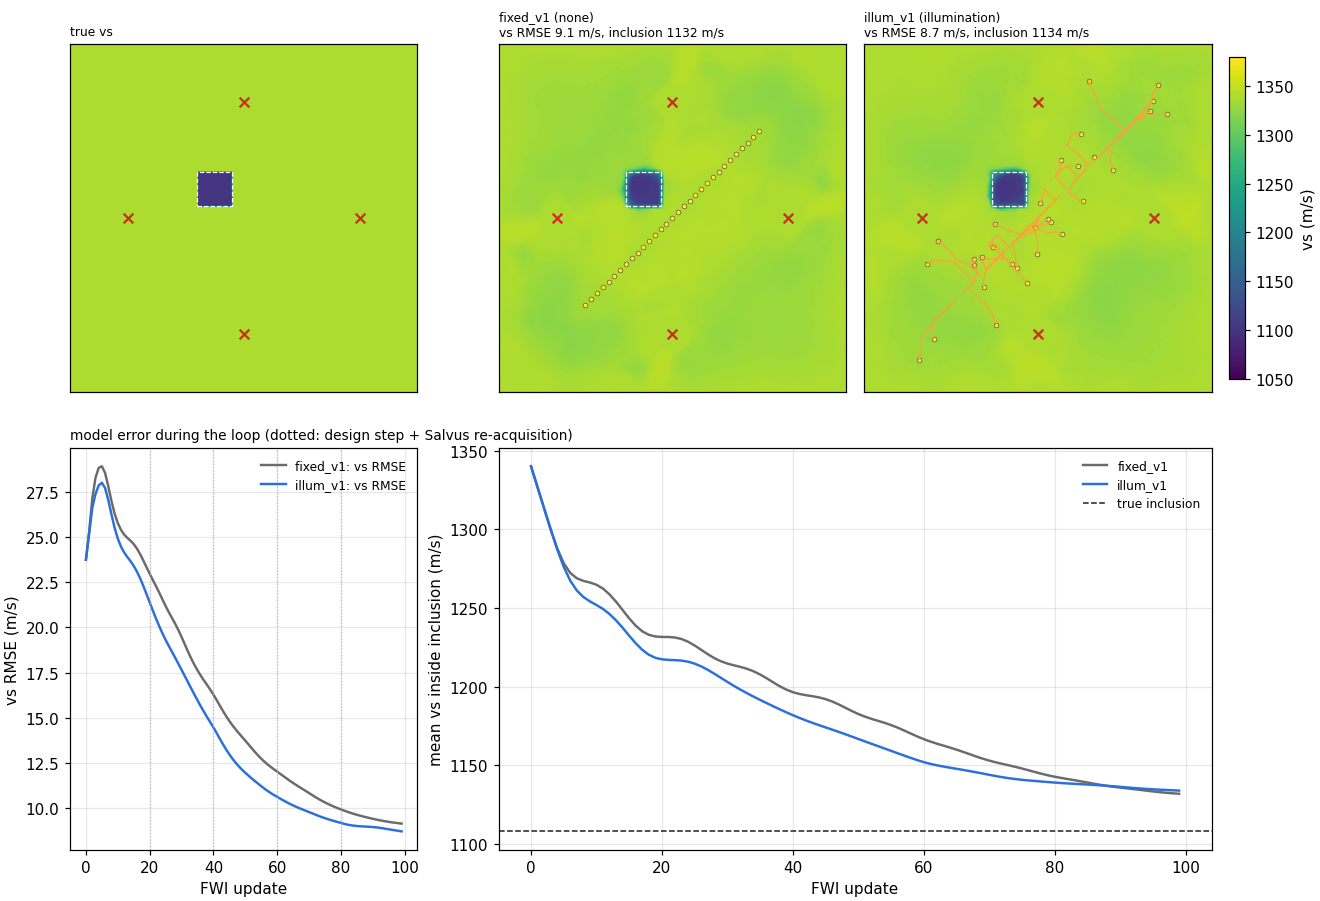
\includegraphics[width=\textwidth]{oed_summary.png}
\caption{Top: true model, fixed layout, illumination-designed layout with receiver trajectories. Bottom: model error
and inclusion velocity against FWI updates (dotted: design step + Salvus re-acquisition).}
\end{figure}

\begin{table}[h]
\centering\small
\resizebox{\textwidth}{!}{\begin{tabular}{@{}lcccc@{}}
\toprule
Layout & vs RMSE after 40 / 60 / 100 updates & Inclusion vs & Wall time & Overhead per round \\
\midrule
Fixed diagonal & 16.3 / 12.0 / 9.1 & 1132 & 11.0 min & -- \\
Illumination OED & 14.5 / 10.6 / 8.7 & 1134 & 13.0 min & 7~s design + 18~s Salvus \\
\bottomrule
\end{tabular}}
\caption{Designed receivers converge faster ($-$11 to $-$12\,\% mid-run); with 100 updates and TV both layouts largely
converge ($-$5\,\% at the end). Single run: no statistics yet.}
\end{table}

\FloatBarrier
%======================================================================
\section{The real LDV data}
\subsection{What the scan contains}
The \code{.mat} file is a Polytec export without plate, source or scatterer metadata (11\,229 points on a 1.5~mm grid,
0.33~m~$\times$~0.11~m, 625~kHz, 1.5~ms).

\begin{figure}[h]
\centering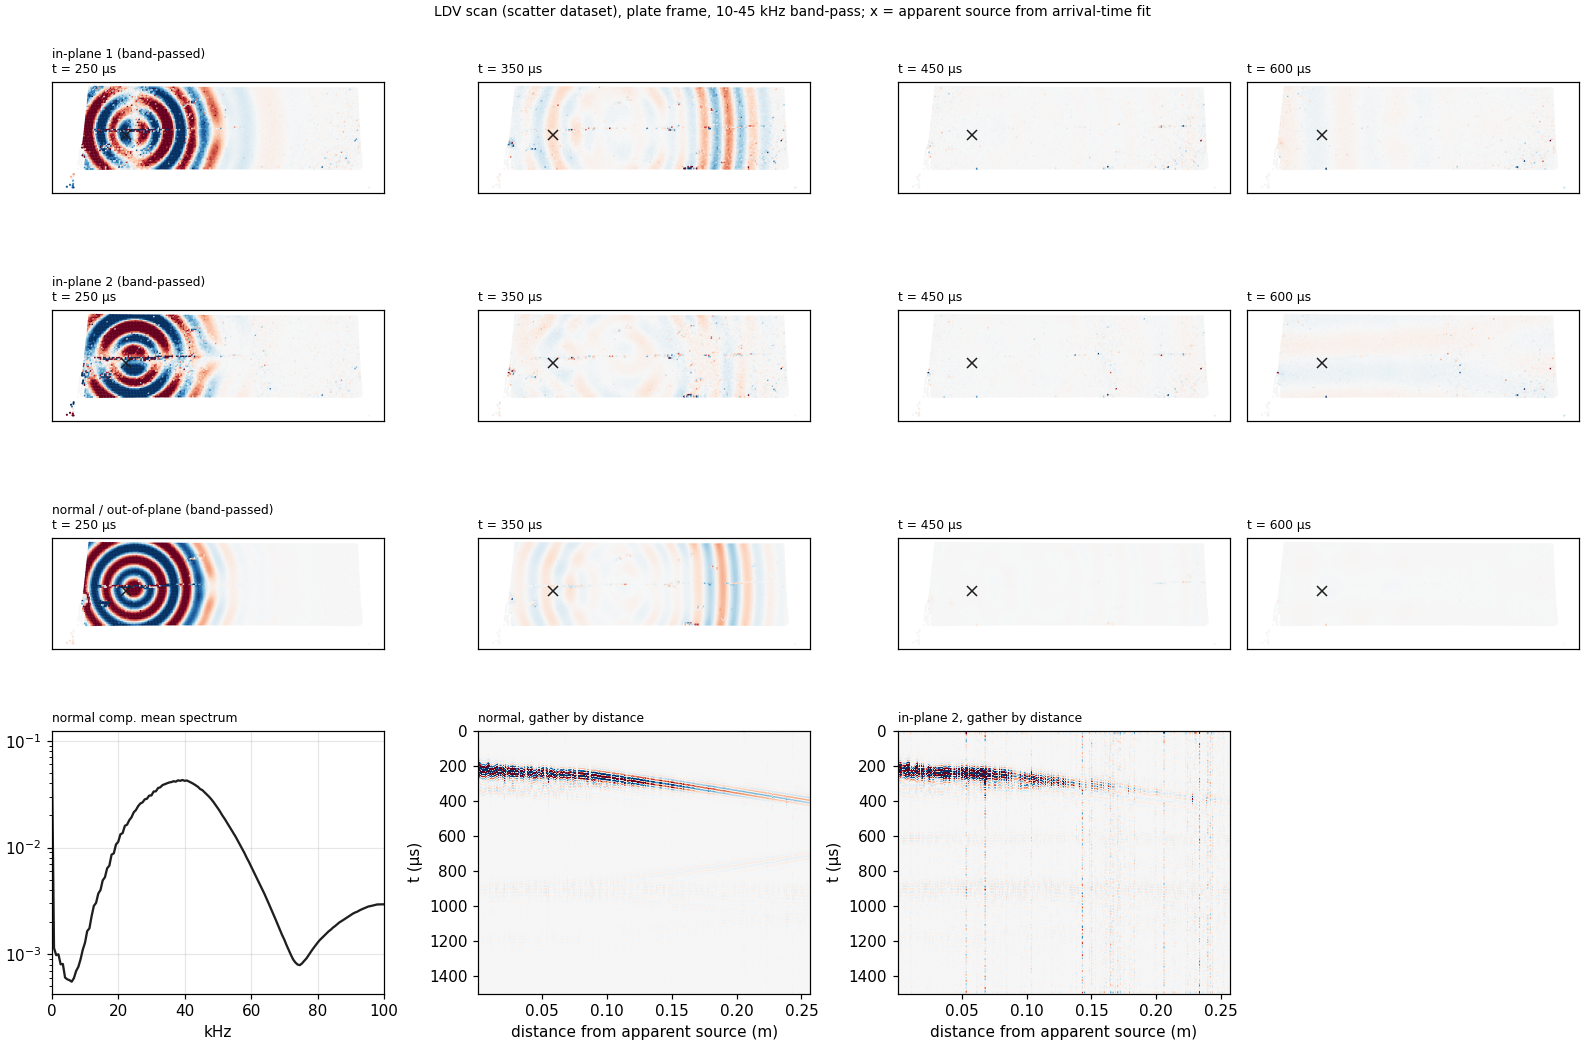
\includegraphics[width=\textwidth]{ldv_components.png}
\caption{Scan rotated into the plate frame. The out-of-plane component is clean (SNR $\approx$ 90 after band-pass);
the two in-plane channels show the same rings with the same sign as the out-of-plane field (cross-talk, not radial
in-plane motion) plus dropouts. The energy travels at $\approx$1320~m/s, the A0 group velocity of 10~mm PMMA at the
39~kHz spectral peak. Trigger delay $\approx$170--200~$\mu$s.}
\end{figure}

Consequence: plane stress cannot be used for this data; the forward model must be flexural (Mindlin).

\subsection{Explaining the scan: steel cube and attenuation}
A homogeneous Mindlin plate reproduced the wave timing and dispersion but left a sharp shadow cone and a reflected
bump on the source axis. With the information that the plate carries a bonded 10~mm steel cube, a Salvus 3-D model of
the experiment (cube meshed on top of the plate, PMMA with constant Q) located it at $(-20, -5)$~mm in the scan frame
and gave Q~$\approx$~40.

\begin{figure}[h]
\centering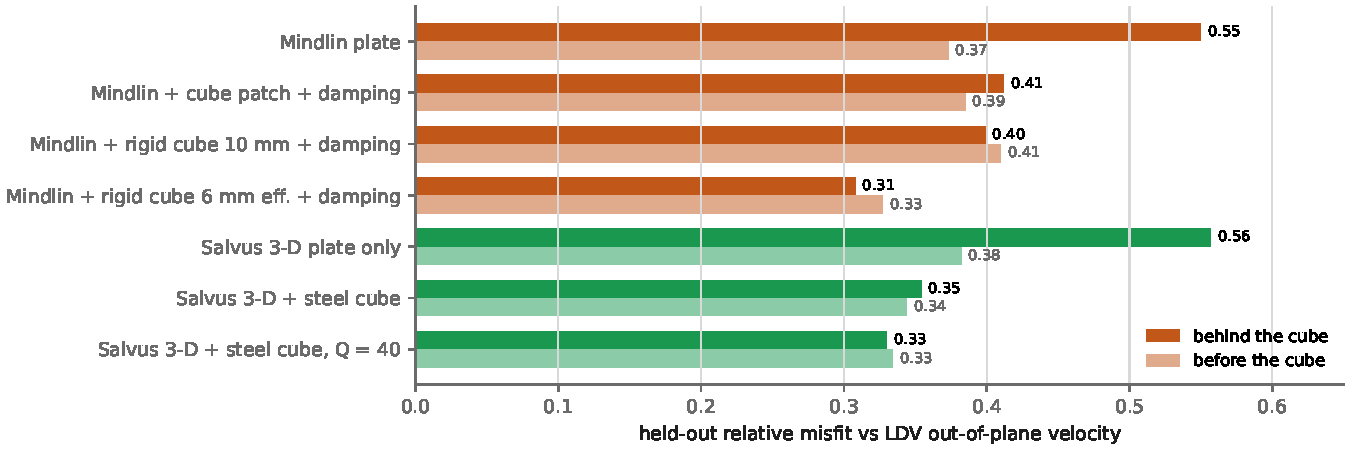
\includegraphics[width=\textwidth]{ldv_models.pdf}
\caption{Held-out misfit against the LDV out-of-plane velocity, behind and before the cube (near-source zone and a bad
scan row excluded; one deconvolution filter per model estimates the source wavelet and trigger delay).}
\end{figure}

\subsection{A fast Mindlin equivalent}
Two Mindlin representations of the cube were tested. A stiffened patch with the physical mass ($\times$7.65) and
rotary inertia ($\times$87.5) rang at a spurious resonance. A rigid-body constraint (footprint moves as deflection
plus two rotations, carrying the cube's mass and rotary inertia about the mid-plane) removes the resonance; its single
free parameter, the effective footprint, was calibrated against Salvus only.

\begin{figure}[h]
\centering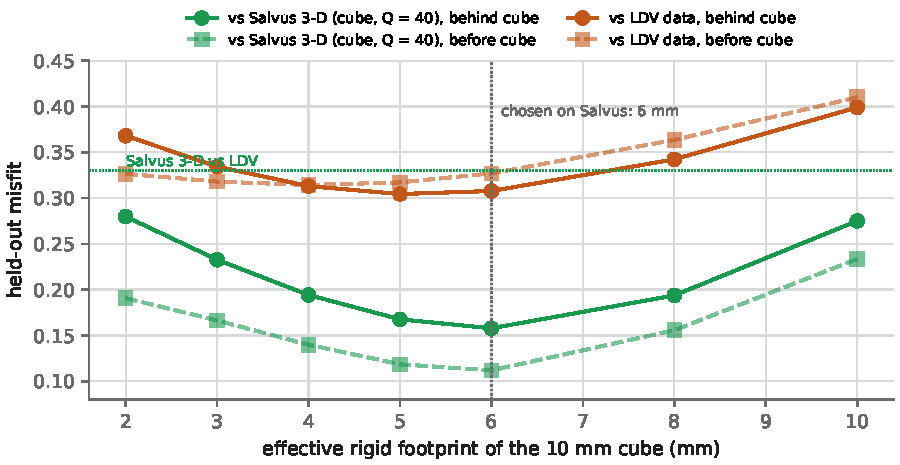
\includegraphics[width=0.75\textwidth]{rigid_footprint.pdf}
\caption{Calibration of the rigid footprint. A 6~mm effective footprint for the 10~mm cube is best against Salvus
(0.16/0.11, at the plate-theory limit) and nearly best against the LDV data (0.31/0.33), without tuning on the
data. Halving the cube's rotary inertia made every footprint worse: the cube's rocking is what scatters A0.}
\end{figure}

\begin{figure}[h]
\centering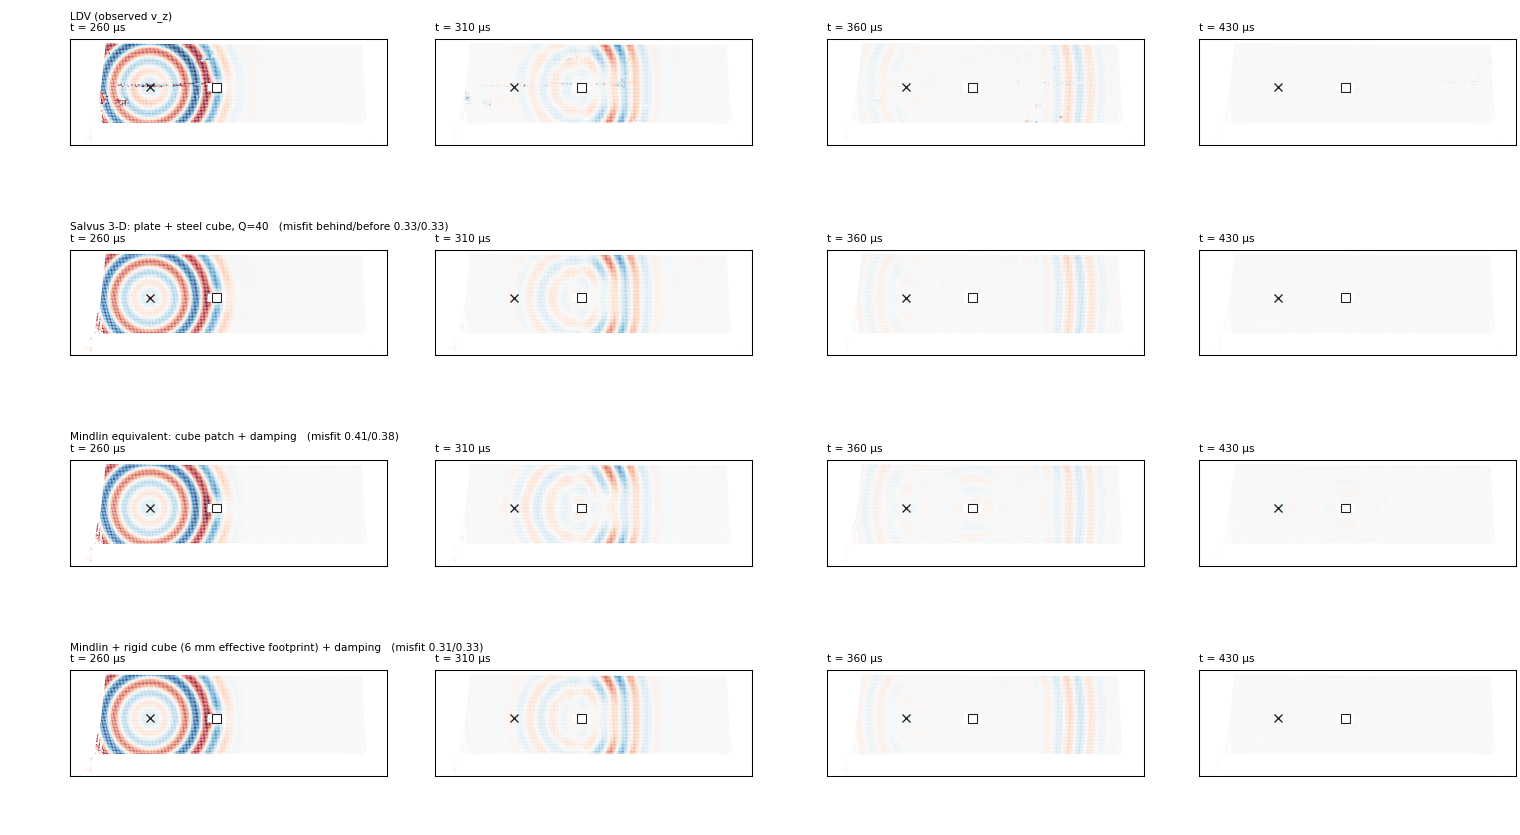
\includegraphics[width=\textwidth]{ldv_snapshots.png}
\caption{Snapshots: LDV, Salvus 3-D (cube, Q = 40), Mindlin patch equivalent, Mindlin rigid cube (square: cube,
cross: transducer).}
\end{figure}

\begin{figure}[h]
\centering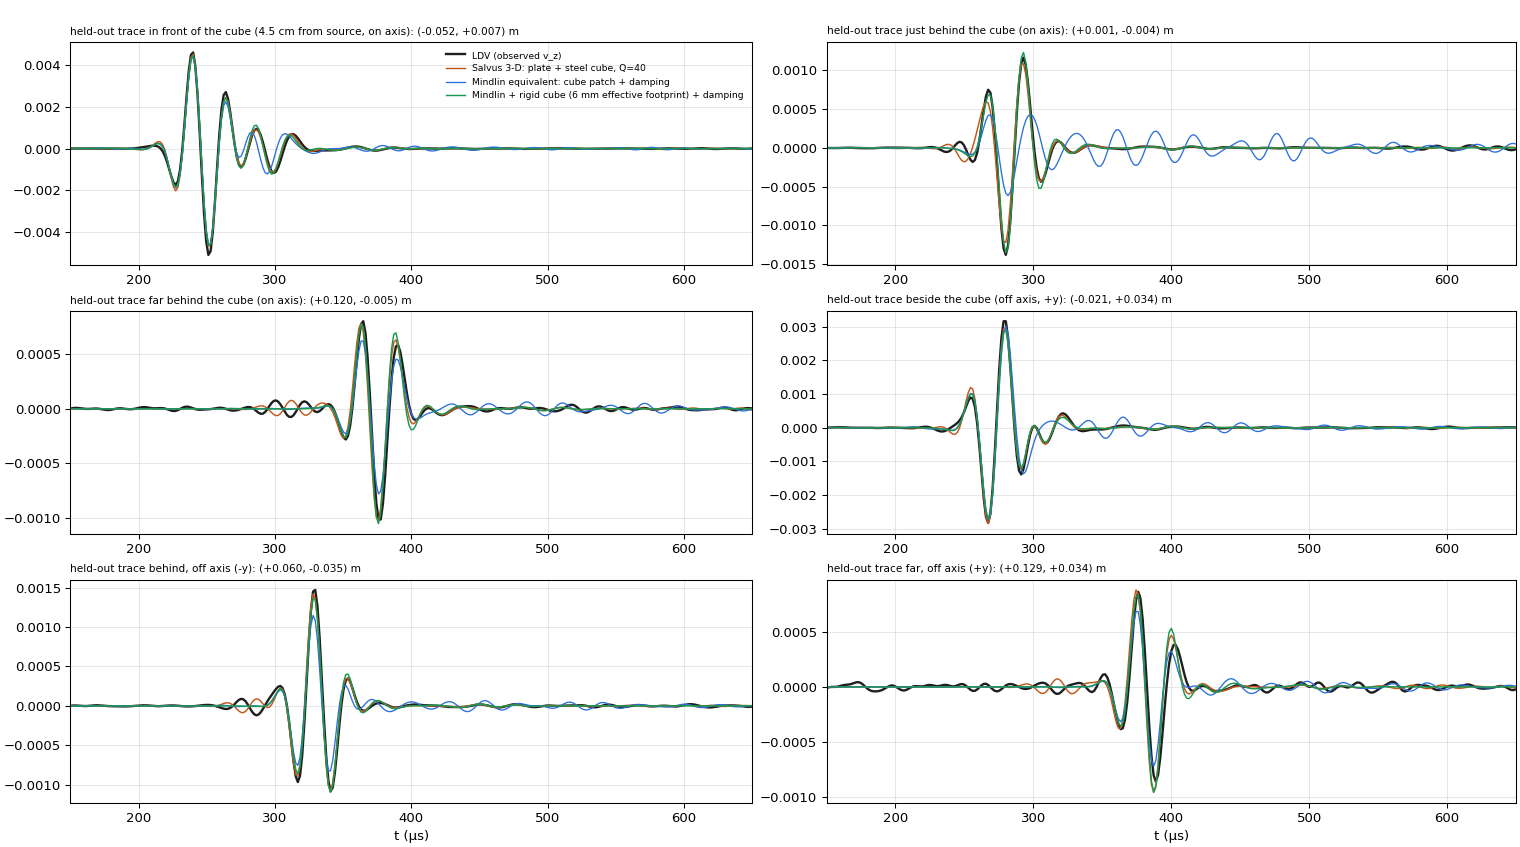
\includegraphics[width=\textwidth]{ldv_traces.png}
\caption{Held-out traces (black: LDV, orange: Salvus 3-D, blue: Mindlin patch, green: Mindlin rigid cube). The rigid
cube follows the data in front of, behind and beside the cube; the patch rings behind it.}
\end{figure}

\FloatBarrier

%======================================================================
\section{OED on the LDV setup}\label{sec:oed-ldv}
This section moves the loop from the synthetic Salvus benchmark to the actual LDV experiment: the same plate, transducer
position and scan area, out-of-plane velocity, and the Mindlin plate solver (damping, $\kappa$ matched to A0) as the
forward model of the FWI.

\subsection{Static FWI on the full scan}
Before any design, the full scan was inverted directly (half of the 11k points for fitting, half held out).
\begin{itemize}
  \item \textbf{Parametric search} (rigid cube on a 1~mm grid): the best position is ($-18$, $-4$)~mm, 2~mm from the
        Salvus 3-D fit. Held-out misfit 0.62, against 0.82 for the plain plate.
  \item \textbf{Blind map} (log mass and rotary-inertia scale on a 2.5~mm grid, TV, no cube prior): the held-out misfit
        behind the cube falls from 0.48 to 0.28, slightly better than the parametric cube (0.31). The mass map puts
        a compact anomaly at the cube. A second anomaly appears at the left edge of the scan ($x\approx-150$~mm),
        and the rotary inertia absorbs smooth, large-scale misfit.
\end{itemize}
This is why the OED loop below inverts only the mass map. It also flags \textbf{scan-edge artefacts}, which come back
in the replay lab.

\begin{figure}[h]
\centering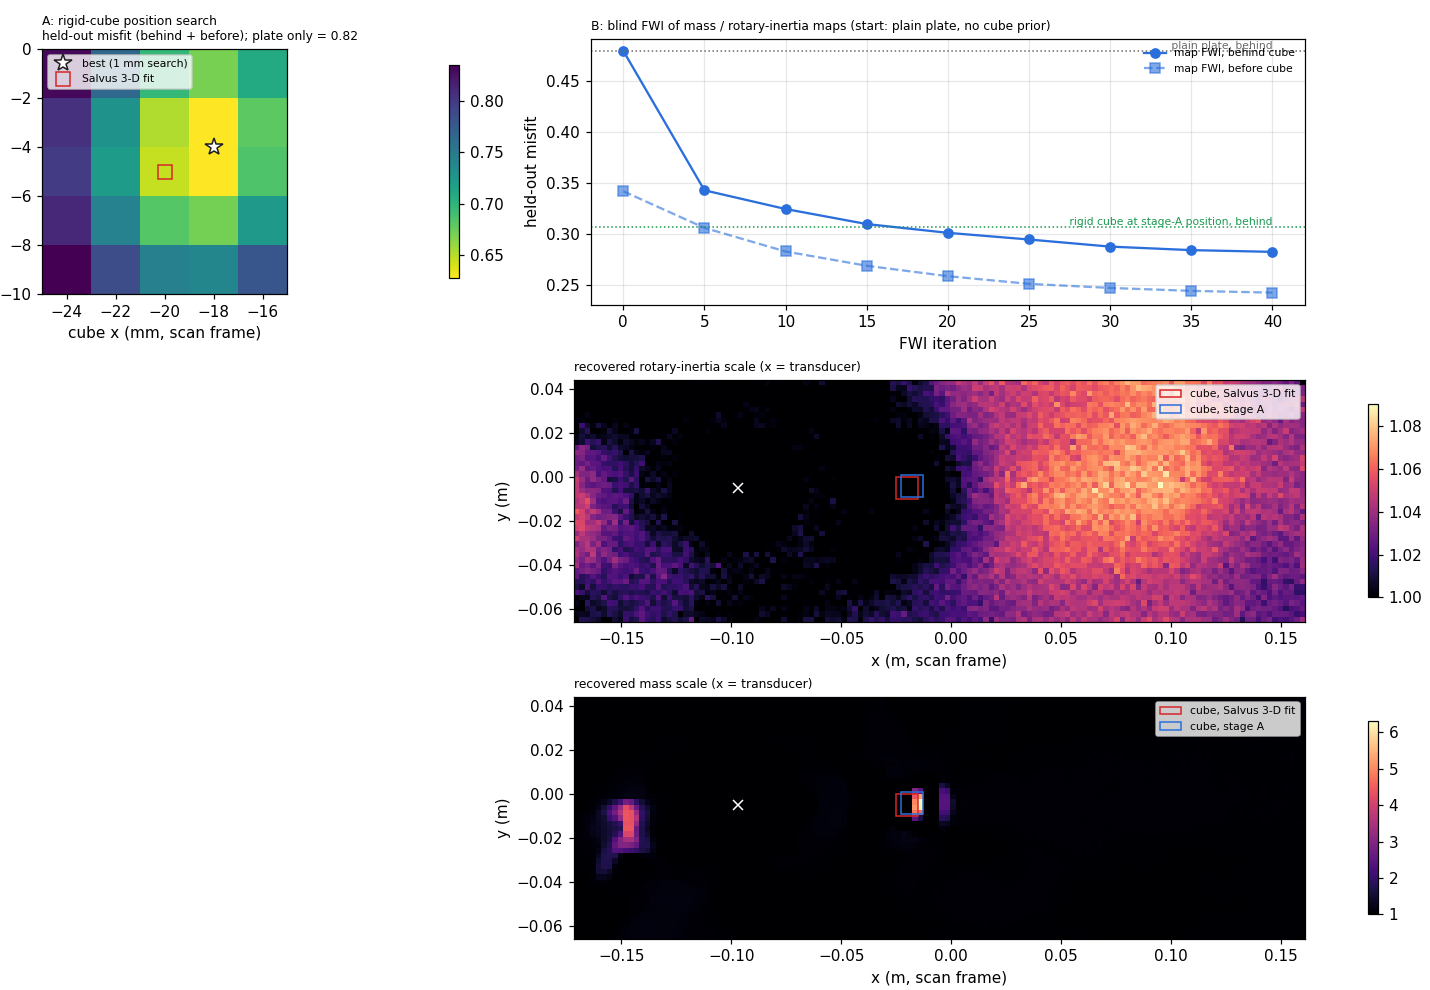
\includegraphics[width=\textwidth]{ldv_static_fwi.png}
\caption{Static FWI on the full LDV scan. A: held-out misfit of the rigid-cube position search. B: held-out misfit
during the blind map FWI, recovered rotary-inertia and mass maps (red: Salvus cube fit; blue: position from A).}
\end{figure}

\subsection{The online loop and the three labs}
Each round follows the order of the lab: \textbf{acquire} at the current points $\to$ \textbf{10 FWI updates}
(Adam, mass map, Mindlin on a 0.5~mm grid) $\to$ \textbf{design step} (illumination on a 1~mm grid, one Adam step on
the point coordinates). Five rounds, 30 LDV points starting on a line at $y=40$~mm. Points are kept inside the scan
area and outside 4~cm of the transducer. The baseline keeps the starting line for all five rounds (same 50 FWI
updates). Only the lab, i.e.\ what an ``acquisition'' returns, changes:

\begin{table}[h]
\centering\small
\begin{tabularx}{\textwidth}{@{}p{2.6cm}Lp{3.2cm}@{}}
\toprule
Lab & Observed data at the requested points & Cost per acquisition \\
\midrule
Mindlin lab & Calibrated Mindlin plate with the rigid steel cube at ($-20$, $-5$)~mm, a different wavelet and trigger delay. Same physics as the FWI: no model error. & $\sim$5~s \\
Salvus 3-D lab & New Salvus simulation of the 3-D plate with the bonded steel cube and Q~=~40: model error similar to real data, no noise. & $\sim$3~min (GPU) \\
Replay lab & \textbf{Real LDV traces}: the nearest point of the dense scan (1.5~mm grid; points within 4~cm of the transducer and on the scan row through it are excluded). The FWI uses the snapped positions. Truth for scoring: the cube at ($-18$, $-4$)~mm from the static search. & none (lookup) \\
\bottomrule
\end{tabularx}
\end{table}
The FWI never sees the lab's wavelet, delay or cube model. The source filter is estimated in closed form at every
update. In every lab the measured data are constants in the hypergradient, as they would be in the lab.

\begin{figure}[h]
\centering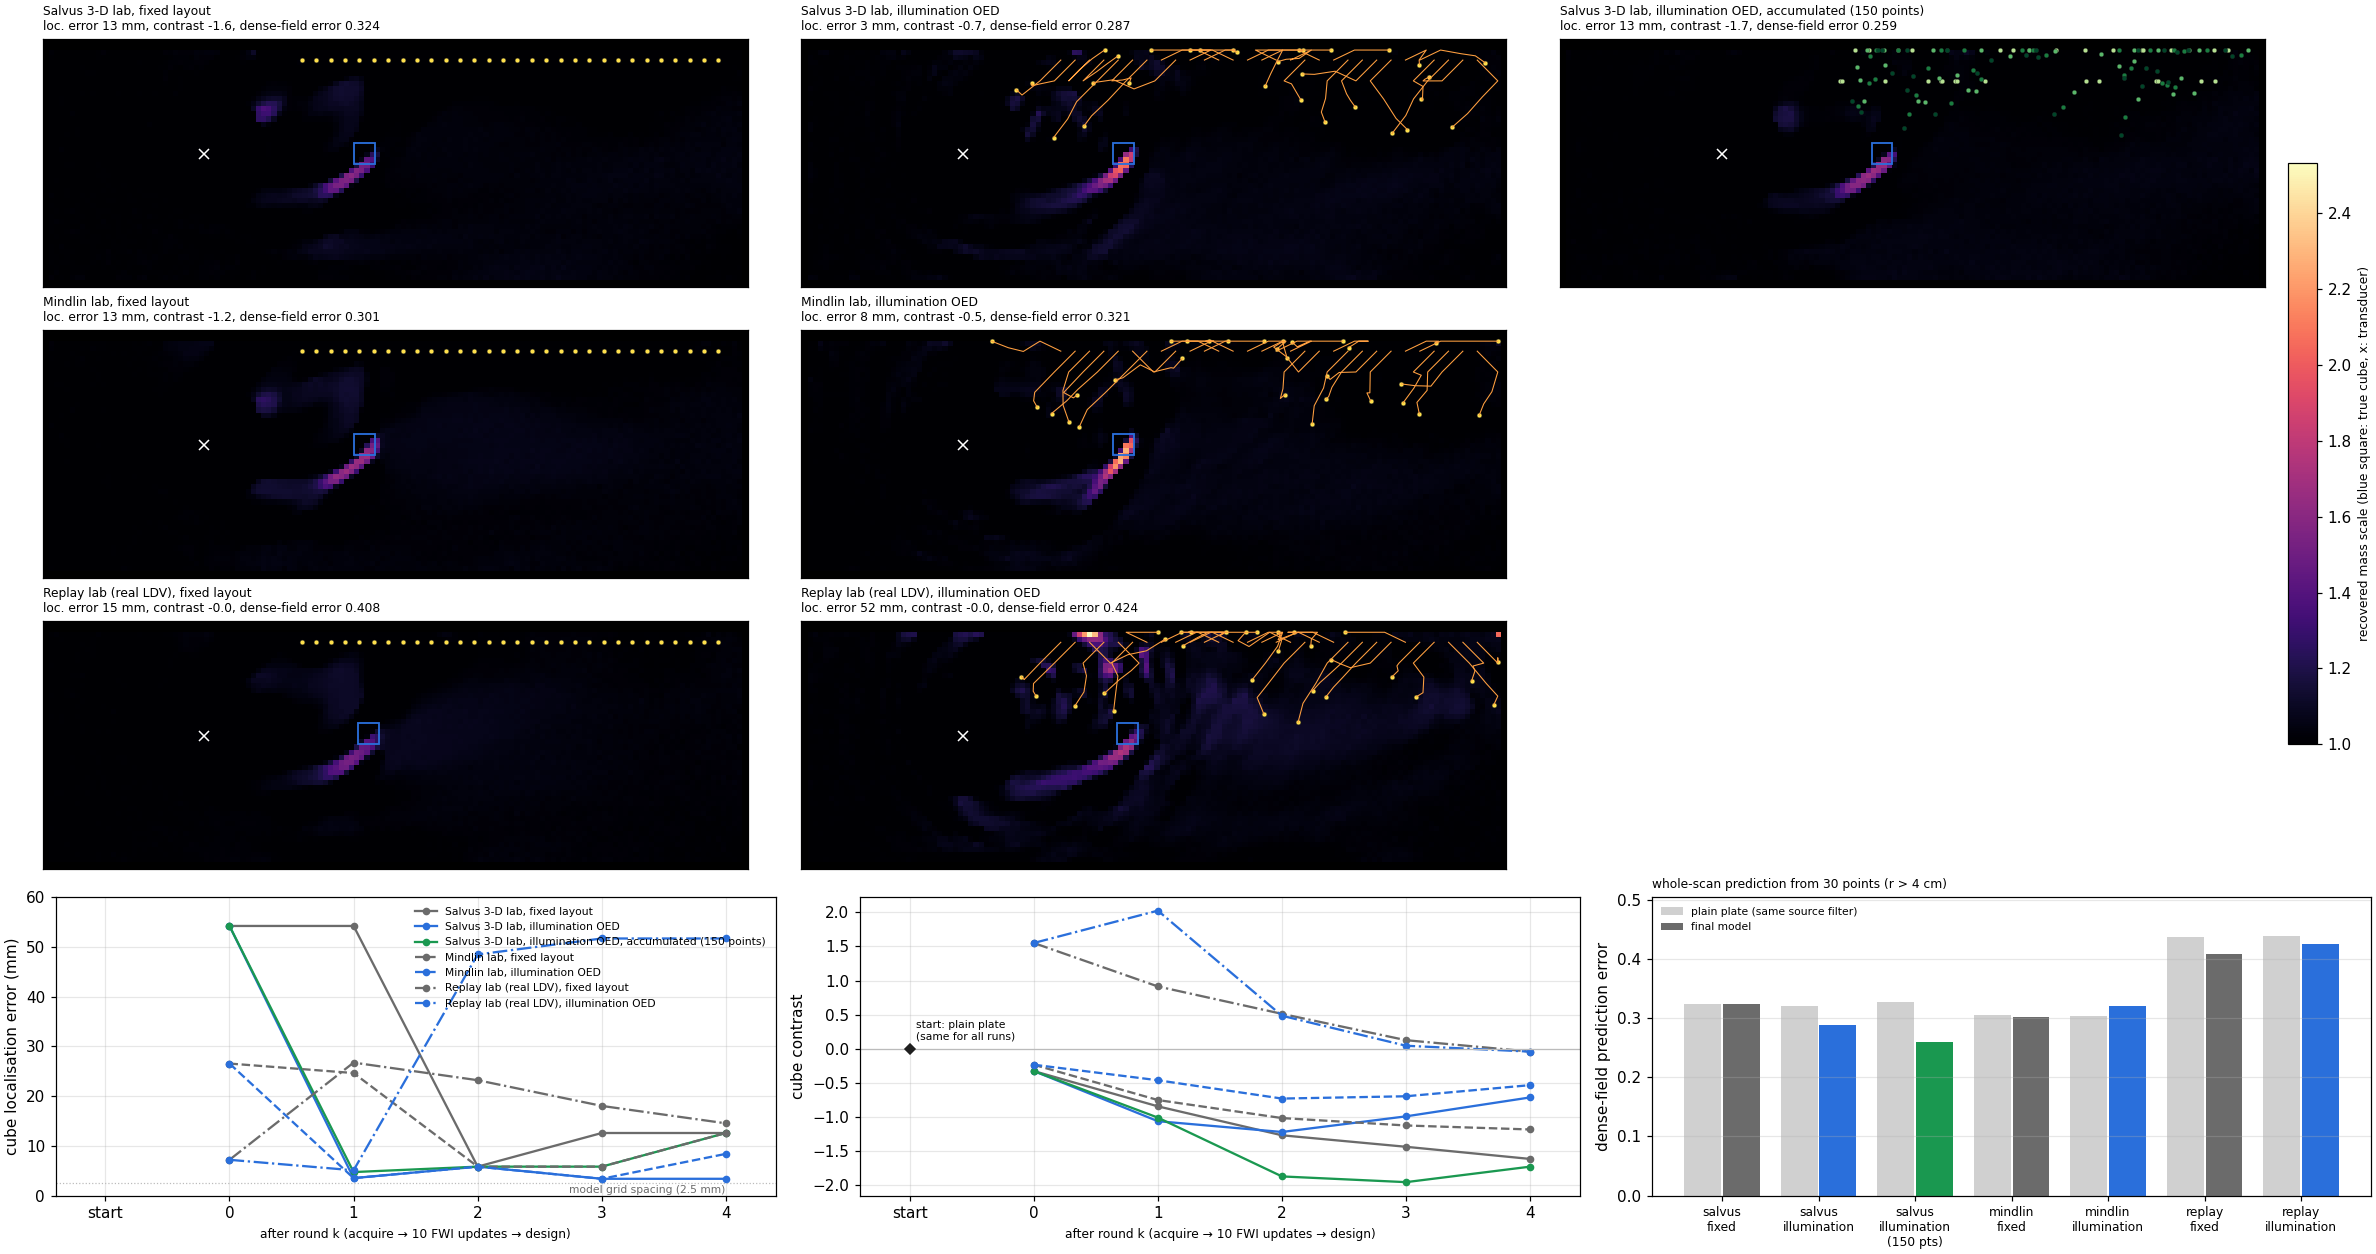
\includegraphics[width=\textwidth]{oed_ldv_all.png}
\caption{Recovered mass maps after five rounds (rows: labs; columns: fixed line, illumination OED, illumination with
all 150 measured points kept). Orange: point trajectories; yellow: final points; blue square: true cube; $\times$:
transducer. Bottom: cube localisation error (peak of the mass map) and contrast per round, and the error when the
final model predicts the whole scan ($r>4$~cm).}
\end{figure}

\begin{table}[h]
\centering\small
\resizebox{\textwidth}{!}{\begin{tabular}{@{}llccccc@{}}
\toprule
Lab & Layout & Loc.\ error & Best round & Mass at cube & Strongest anomaly & Whole-scan error (plain) \\
\midrule
Mindlin & fixed & 12.6~mm & 5.8 & $\times$1.61 & $\times$1.67 & 0.301 (0.305) \\
        & illumination & 8.4~mm & 3.4 & $\times$\textbf{2.29} & $\times$2.29 & 0.321 (0.303) \\
\midrule
Salvus 3-D & fixed & 12.6~mm & 5.8 & $\times$1.43 & $\times$1.60 & 0.324 (0.323) \\
           & illumination & \textbf{3.4~mm} & 3.4 & $\times$\textbf{2.10} & $\times$2.10 & 0.287 (0.321) \\
           & illumination, 150 pts & 12.6~mm & 4.8 & $\times$1.60 & $\times$1.66 & \textbf{0.259} (0.326) \\
\midrule
Replay (real) & fixed & 14.5~mm & 7.2 & $\times$1.40 & $\times$1.53 & 0.408 (0.437) \\
              & illumination & 51.7~mm & 5.1 & $\times$\textbf{1.63} & $\times$2.53 & 0.424 (0.438) \\
\bottomrule
\end{tabular}}
\caption{Final metrics after five rounds (single run each). Localisation error: distance from the mass-map peak
to the true cube. Best round: smallest localisation error over the five rounds. Mass at cube: largest recovered mass scale inside the 10~mm cube
square. Strongest anomaly: largest mass scale anywhere; when it exceeds the mass at the cube, the peak is a spurious
anomaly. Runs take 11--13~min (26~min with Salvus re-acquisition); the design step takes about 12~s.}
\end{table}

\subsection{General comments}
\begin{itemize}
  \item \textbf{The machinery is ready for the lab.} The loop runs end to end on real data with the order and data flow
        of the experiment: measured traces enter only as constants, the wavelet and trigger delay are estimated, and
        a design step costs about 12~s. The remaining work is mostly experimental, not computational.
  \item \textbf{Consistent effect of illumination:} in all three labs the designed points put more recovered mass at the
        cube ($\times$1.43 $\to$ 2.10 Salvus, 1.61 $\to$ 2.29 Mindlin, 1.40 $\to$ 1.63 real data), i.e.\ the defect is
        imaged more strongly. The designed points move down from the starting line towards the region behind and
        beside the cube.
  \item \textbf{The single transducer limits what any layout can do.} All maps show a streak along the source--cube
        line: with one source the travel-time information does not separate range from scattering strength. The peak
        then slides along the streak, which explains most of the 5--13~mm errors. A second or third transducer position
        should help more than any point layout.
  \item \textbf{Real data add spurious anomalies at the scan edge.} In the replay lab the designed points crowd onto the
        top edge of the scan ($y=45$~mm), and the FWI builds a mass anomaly there ($\times$2.5) that takes the peak,
        hence the 52~mm error, although the cube itself is better imaged. The static FWI shows a similar artefact at the
        left edge. Probable causes: edge data quality, the transducer near field, or physics missing from the model
        (plate edges and supports outside the scan are unknown). A defect-free reference scan would tell.
  \item \textbf{Localisation from one peak is fragile}, and the contrast metric is negative whenever the anomaly is a
        streak. Better metrics (mass or energy inside the defect, the peak of a smoothed map, error in defect size) and
        several seeds per configuration are needed before claiming a gain.
  \item \textbf{Keeping old data} (150 points) gives the best whole-scan prediction (0.259) but not better localisation.
        The fair comparison is at equal measurement budget, i.e.\ against 150 fixed points or a dense scan.
  \item \textbf{Objectives:} the lab-consistent waveform-misfit objective was tested and dropped. It moved points away
        from the scatterer (23~mm localisation error in both labs). Illumination is the objective to keep.
  \item \textbf{The steel cube is an easy target.} It is a strong, compact scatterer, so even the fixed line finds it to
        within $\sim$1.5~cm. OED should matter more for a weak, realistic defect, where the fixed layout may miss it.
\end{itemize}

\subsection{Points for the next experiment}\label{sec:next-experiment}
For discussion with the lab before acquiring new data. The aim is a setup that is realistic for NDT and that the
models can reproduce, with enough ground truth to score the OED.
\begin{itemize}
  \item \textbf{Defect.} Replace the bonded cube with machined, NDT-relevant defects of known geometry: a flat-bottom
        hole or local thickness loss (corrosion-like), possibly a notch, or a small bonded patch as a weak scatterer.
        Ideally use two defect sizes or depths, so detectability can be studied.
  \item \textbf{Reference scan.} Scan the same plate before machining the defect, or a twin plate. This gives a
        defect-free baseline: material calibration (velocity, thickness, damping), and it separates
        defect scattering from edge or near-field effects.
  \item \textbf{Several transducer positions.} Use two or three source positions around the defect, scanned in turn
        (or one source per round in the loop). This is expected to remove the source--defect streak.
  \item \textbf{Metadata to record.} For each acquisition, record:
        \begin{itemize}
          \item plate size, thickness map, material and support or edge conditions;
          \item transducer type, size, coupling and exact position;
          \item excitation signal and the recorded drive or trigger signal;
          \item scan grid in plate coordinates (registration);
          \item sampling rate, record length, number of averages, and the LDV signal level or dropout flag per point;
          \item temperature.
        \end{itemize}
  \item \textbf{Scan area.} The defect should be well inside the scanned area (at least 3--4~cm from the scan edges,
        given the edge artefacts) and far from the transducer: the 4~cm around it are excluded. Record long enough to
        include the first plate-edge reflections, or keep the edges far away. The 1.5~mm grid of the current scan is
        sufficient.
  \item \textbf{Signal.} The out-of-plane channel is all that is used: a 1-D LDV is sufficient. A broadband pulse
        (current: about 8--70~kHz) works well with the closed-form wavelet estimate.
  \item \textbf{Repeatability.} Re-measure a few points at the start and end of a session, to quantify drift. This
        decides whether data from earlier rounds can be accumulated.
  \item \textbf{Automation (for the live loop).} The PSV must accept a list of arbitrary points from a script and return
        the traces. We also need the measurement time per point (averaging, mirror travel), which sets the cost of a
        round and the measurement-time term of the design.
  \item \textbf{Dense scans remain useful.} A full dense scan of each new configuration doubles as a replay lab and as
        the reference for ``how many points does the loop need to match the full scan''.
\end{itemize}

\FloatBarrier
%======================================================================
\section{Caveats and open methodological points}
\begin{itemize}
  \item \textbf{OED evidence is thin:} one run per configuration, one target (a strong scatterer), one source. Gains
        show as faster convergence and stronger imaging of the defect, not yet as robust localisation.
  \item \textbf{Metrics:} the mass-map peak is fragile against spurious anomalies, and the contrast metric is negative for
        streak-like anomalies. Both should be replaced before a multi-seed study.
  \item \textbf{Hypergradients with measured data:} the synthetic runs of the paper differentiate through
        $d_{\mathrm{obs}}(\mathbf p)$ (computed with the true model). In the lab the data are constants; the
        waveform-misfit and oracle objectives must be re-derived and re-tested without that term. Illumination is
        unaffected.
  \item \textbf{Plate theories are approximations:} plane stress ignores S0 dispersion (corrected at one frequency);
        Mindlin needs a calibrated $\kappa$, a 0.5~mm grid, and misses the weak symmetric part of a surface load.
        Damping is velocity-proportional, not constant Q.
  \item \textbf{LDV specifics:} only the out-of-plane channel is usable; the transducer near field is not modelled
        (most of the remaining residual is within 4~cm of the source); one scan row has dropouts.
  \item \textbf{Tooling:} Salvus runs from a version-matched venv (binary 2025.1.2, conda package 2025.1.1); constant Q
        uses a private Salvus helper; Salvus events must be launched with sorted names (a permutation bug was found
        and fixed).
\end{itemize}

%======================================================================
\section{What remains for OED with the LDV in the loop}
\begin{table}[h]
\centering\small
\begin{tabularx}{\textwidth}{@{}p{3.6cm}Lp{2.2cm}@{}}
\toprule
Item & What is needed & Status \\
\midrule
Forward model for the lab & Mindlin + damping + rigid attachments (done); thickness map $h(x,y)$ as a defect parameter; finite-transducer source. & mostly done \\
Inversion on real data & Static Mindlin FWI on the full scan: cube position (done), blind mass map (done, edge artefact); thickness or stiffness maps for realistic defects. & partly done \\
Replay lab & The dense scan as the ``instrument'' (nearest measured traces). Built and run; to repeat on new datasets. & done \\
Virtual lab & Salvus 3-D (cube, Q) + an LDV noise model (SNR per point, dropouts) behind the same acquisition interface. & partly (Salvus side done) \\
Lab-consistent objectives & Illumination (used); waveform misfit with constant measured data (tested, dropped); measurement-cost terms (points, averaging, travel, excluded zones). & partly \\
Experimental setup & Realistic defect, several transducer positions, reference scan, metadata (Section~\ref{sec:next-experiment}). & to discuss \\
Source and calibration & Wavelet and trigger delay estimated inside the loop; scan-to-plate registration; plate size and edges; material ($v_s$, $h$, Q). & partly \\
Instrument integration & Polytec PSV automation: arbitrary point lists, triggering, data return; latency budget per round (minutes). & to do \\
New datasets & Your upcoming scans with full metadata (transducer, plate, defect, scan position). & pending \\
\bottomrule
\end{tabularx}
\end{table}

\section{From proof of concept to an application paper}
\begin{itemize}
  \item \textbf{Claim:} online OED reaches the same defect localisation and characterisation as a full LDV grid scan
        with far fewer points and less scan time (a full scan is 11k points $\times$ 100 averages).
  \item \textbf{Metrics:} defect position, size and mass error and detection probability against number of points and
        scan time, not only model MSE.
  \item \textbf{Baselines:} full grid scan (reference), uniform sparse grids, random layouts, greedy sequential OED from
        a candidate set, fixed layouts.
  \item \textbf{Experiments:} (1) virtual lab, many seeds and defect types (bonded masses, thickness loss / flat-bottom
        holes, stiffness changes); (2) replay lab on dense LDV scans; (3) live LDV closed loop.
  \item \textbf{Venues:} NDT\&E International, Ultrasonics, Mechanical Systems and Signal Processing, Structural Health
        Monitoring. The method transfers to adaptive seismic acquisition and SHM sensor placement.
  \item \textbf{Before writing:} package the new code with tests (dispersion vs analytic, free-edge energy, remat
        gradient equality), isolate the private Salvus helper, document the environments.
\end{itemize}

\begin{keybox}{Suggested order of work}
\begin{enumerate}
  \item \emph{Done:} static Mindlin FWI on the full LDV scan (cube position, blind mass map).
  \item \emph{Done:} OED loop on Mindlin with illumination (waveform objective tested and dropped).
  \item \emph{Done (one run):} replay-lab OED on the dense scan against the fixed layout.
  \item \textbf{Now:} design the new experiment with the lab (Section~\ref{sec:next-experiment}); meanwhile model the
        new defect type (thickness loss in Mindlin and Salvus) and replace the localisation metrics.
  \item Virtual-lab multi-seed study (Salvus 3-D + noise) on the new configuration, several sources, more baselines.
  \item Dense scans of the new plate (replay lab), LDV automation, live closed loop.
\end{enumerate}
\end{keybox}

\appendix
\section{Code map}
\begin{table}[h]
\centering\small
\begin{tabularx}{\textwidth}{@{}p{4.6cm}L@{}}
\toprule
Folder & Content \\
\midrule
\code{src/remat/} & Remat subclass of the paper simulation, hypergradient benchmark, GPU multi-seed runner. \\
\code{src/pinn\_feasibility/} & FD references, scattered-field (FB)PINN, diagnostics. \\
\code{src/elastic/} & Plane stress (CPML, free edges), Mindlin (damping, patches, rigid bodies), 3-D FD, comparisons, FWI. \\
\code{src/salvus\_plate/} & Salvus free-plate benchmark (in-plane and flexural events), export. \\
\code{src/oed\_plate/} & Salvus acquisition (``lab''), plate FWI problem, OED loop, figures. \\
\code{src/ldv\_assessment/} & LDV analysis, Mindlin fits, Salvus cube model, Mindlin equivalent, figures. \\
\code{src/ldv\_inversion/} & Static FWI on the LDV scan: rigid-cube search, blind mass/inertia maps. \\
\code{src/oed\_ldv/} & OED loop on the LDV setup: problem, labs (Mindlin, Salvus, replay), runner, figure. \\
\code{reports/2026-10\_status/} & This report (\code{make\_figures.py}, \code{main.tex}). \\
\bottomrule
\end{tabularx}
\end{table}

\end{document}
